The low Reynolds number is called the creeping, or over-damped
regime. Let us generalize slightly the momentum equation
Eq \ref{eq:NS_usual} to a general volumetric external force $\bff$:
\[
  \rho \frac{d\bfu }{dt} =
  - \nabla p 
  + \mu \nabla^2 \bfu
  + \bff .
\]

We may again cast the equation into reduced form, to get
\[
\rho^* \frac{d\bfu^* }{dt^* } =
-  \nabla^* p^*
+  \frac1{\mathrm{Re}} \nabla^{*2} \bfu^* .
+  \bff^* ,
\]
where $\bff^*= L/(\rho_0 u_0^2) \bff$. 

As $\mathbf{Re}$ is very small, the equation will tend to
\[
0 = - \mathrm{Re} \nabla^* p^* + \nabla^2 \bfu^* + \mathrm{Re} \bff^*
.
\]
All time derivatives are gone from the equation! The only time
variation that is sometimes considered is the case in which $\bff^*$
is a explicit function of time. In this case, the velocity field
adapts instantaneously following the changes in external force. Coming
from previous chapters, devoted to cases where intertial effects are
not negligible, this may come as a surprise --- nevertheless, this is
the correct description of a regime which is important in fields such
as microfluidics and the biological physics of small systems (from
small insects down to large molecules).  Mathematically, the resulting
equation is now linear in the velocity, which makes its treatment
simpler.

An objection could be raised regarding why the pressure gradient and
the external force terms are kept in the equation, despite being
multiplied by the Reynolds number. The answer is that they are not
in fact negligible, as an alternative scaling is employed. This is
discussed in the next section.



\subsection{Kolmogorov flow}

In order to get an idea of the features of the flow (typical speed,
time scale, Reynolds number), we may gain some insight from the
solution from Kolmogorov flow.

This is an exact solution of the momentum equations when there is a
periodic applied force in the $x$ direction that depends on $y$ only
\[
\bff = f_0 \cos\left( \frac{2\pi y}{L} \right) \bfe_x .
\]

In this case, the typical length-scale $L_0$ and velocity $u_0$ are
set by the force. The former is clearly $L_0=L$, but the velocity is
actually part of the solution. It is therefore more convenient to
introduce an alternative way to cast the momentum equation in
non-dimensional form. First, dividing by $f_0$ and going to
dimensionless spacial coordinates:
\begin{equation}
\label{eq:Navier-Stokes_nondim1}
\frac{\rho}{f_0}
\frac{d \bfu}{d t} =
\frac\mu{f_0 L^2} (\nabla^*)^2 \bfu
-\frac 1{f_0 L} \nabla^* p + \bff^*(\bfr^*) .
\end{equation}
The viscous term sets the velocity scale: $u_0 = ( f_0 L^2 ) / \mu $.
On the left hand side the total derivative limits the setting of the
time scale: $t_0=L/u_0$. This means the equation may be written as
\[
\frac{\rho L^3 f_0}{\mu^2}
\frac{d \bfu^*}{d t^*} =
(\nabla^*)^2 \bfu^*
-\nabla^* p^* + \bff^*(\bfr^*) ,
\]
or
\begin{equation}
\label{eq:Navier-Stokes_nondim2}
\mathrm{Re}
\frac{d \bfu^*}{d t^*} =
(\nabla^*)^2 \bfu^*
-\nabla^* p^* + \bff^*(\bfr^*) ,
\end{equation}
where we again find the Reynolds number, given as Re=$\rho L^3 f_0 /
\mu^2$.  Notice that the reduced response time is given by the
Reynolds number: a high Reynolds number means a long reduced time to
respond, while a low Reynolds one the response is very rapid, and the
equilibrium solution is reached very fast. Also, the pressure
is

To summarize, the various scales are given by:
\begin{itemize}
\item force $f_0$
\item space $L$ (therefore, the reduced del operator $\nabla^* :=
  L \nabla$),
\item velocity $u_0 = ( f_0 L^2 ) / \mu $,
\item time $t_0 = L / u_0 = \mu / (f_0 L) $,
\item pressure $p_0= f_0 L $,
\item the Reynolds number is Re=$\rho L^3 f_0 / \mu^2$
\end{itemize}


Let us apply this scaling to the Kolmogorov flow. The starting
equation for the $x$ component of the velocity, called customarily
``$u$'' is:
\begin{equation}
\label{eq:Kolmo_orig}
  \rho \frac{\partial u}{\partial t} =
  \mu \nabla^2 u - \nabla p +   f_0 \cos(2\pi y/L)  .
\end{equation}

We have supposed that the resulting velocity, as the driving force,
only has an $x$ component varying on $y$, so that the convective term
is zero. In this case, the flow is always incompressible
($\nabla\cdot\bfu =0$), so we may set the pressure to some constant
values, which thus disappears from the equation, which is just:
\[
  \rho \frac{\partial u}{\partial t} =
  \mu \nabla^2 u +   f_0 \cos(2\pi y/L)  .
\]

In reduced units (dropping the asterisks for clarity), this is
\[
  \mathrm{Re} \frac{\partial u}{\partial t} = \nabla^2 u + \cos(2\pi y) .
\]

The solution is easily found:
\[
u = \frac{1}{(2\pi)^2} \left( 1-e^{ - (2\pi)^2 t/Re } \right)  \cos(2\pi y) .
\]

Putting the scales back in, we find
\[
u = \frac{ f_0 L^2 }{(2\pi)^2 \mu}
\left( 1-e^{- (2\pi)^2 \mu  t / (\rho L^2) } \right)  \cos(2\pi y/L) ,
\]
which indeed is the solution to the original Equation
\ref{eq:Kolmo_orig}.



\subsection{Creeping flow past objects}



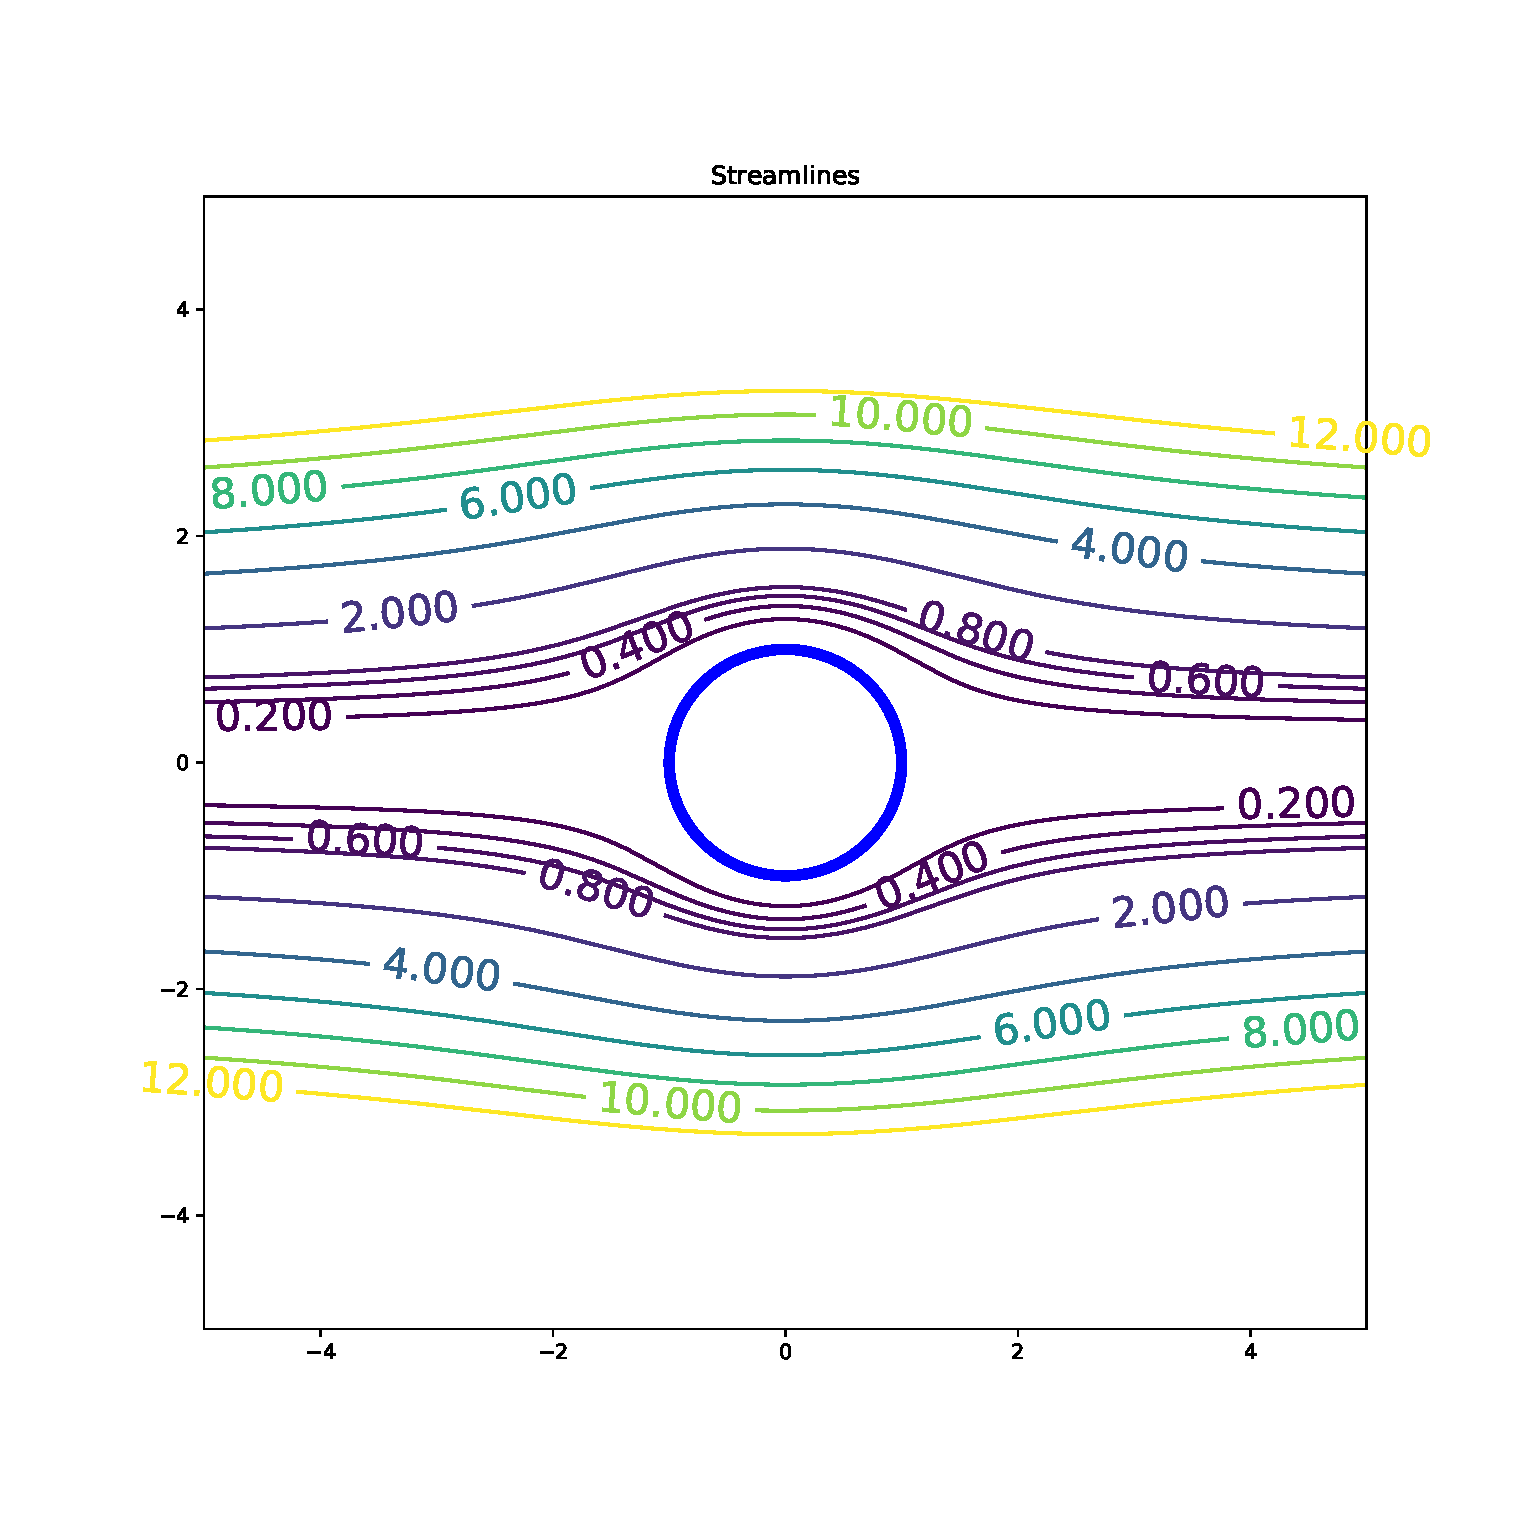
\includegraphics[width=0.8\linewidth]{figures/creeping_flow_past_sphere}

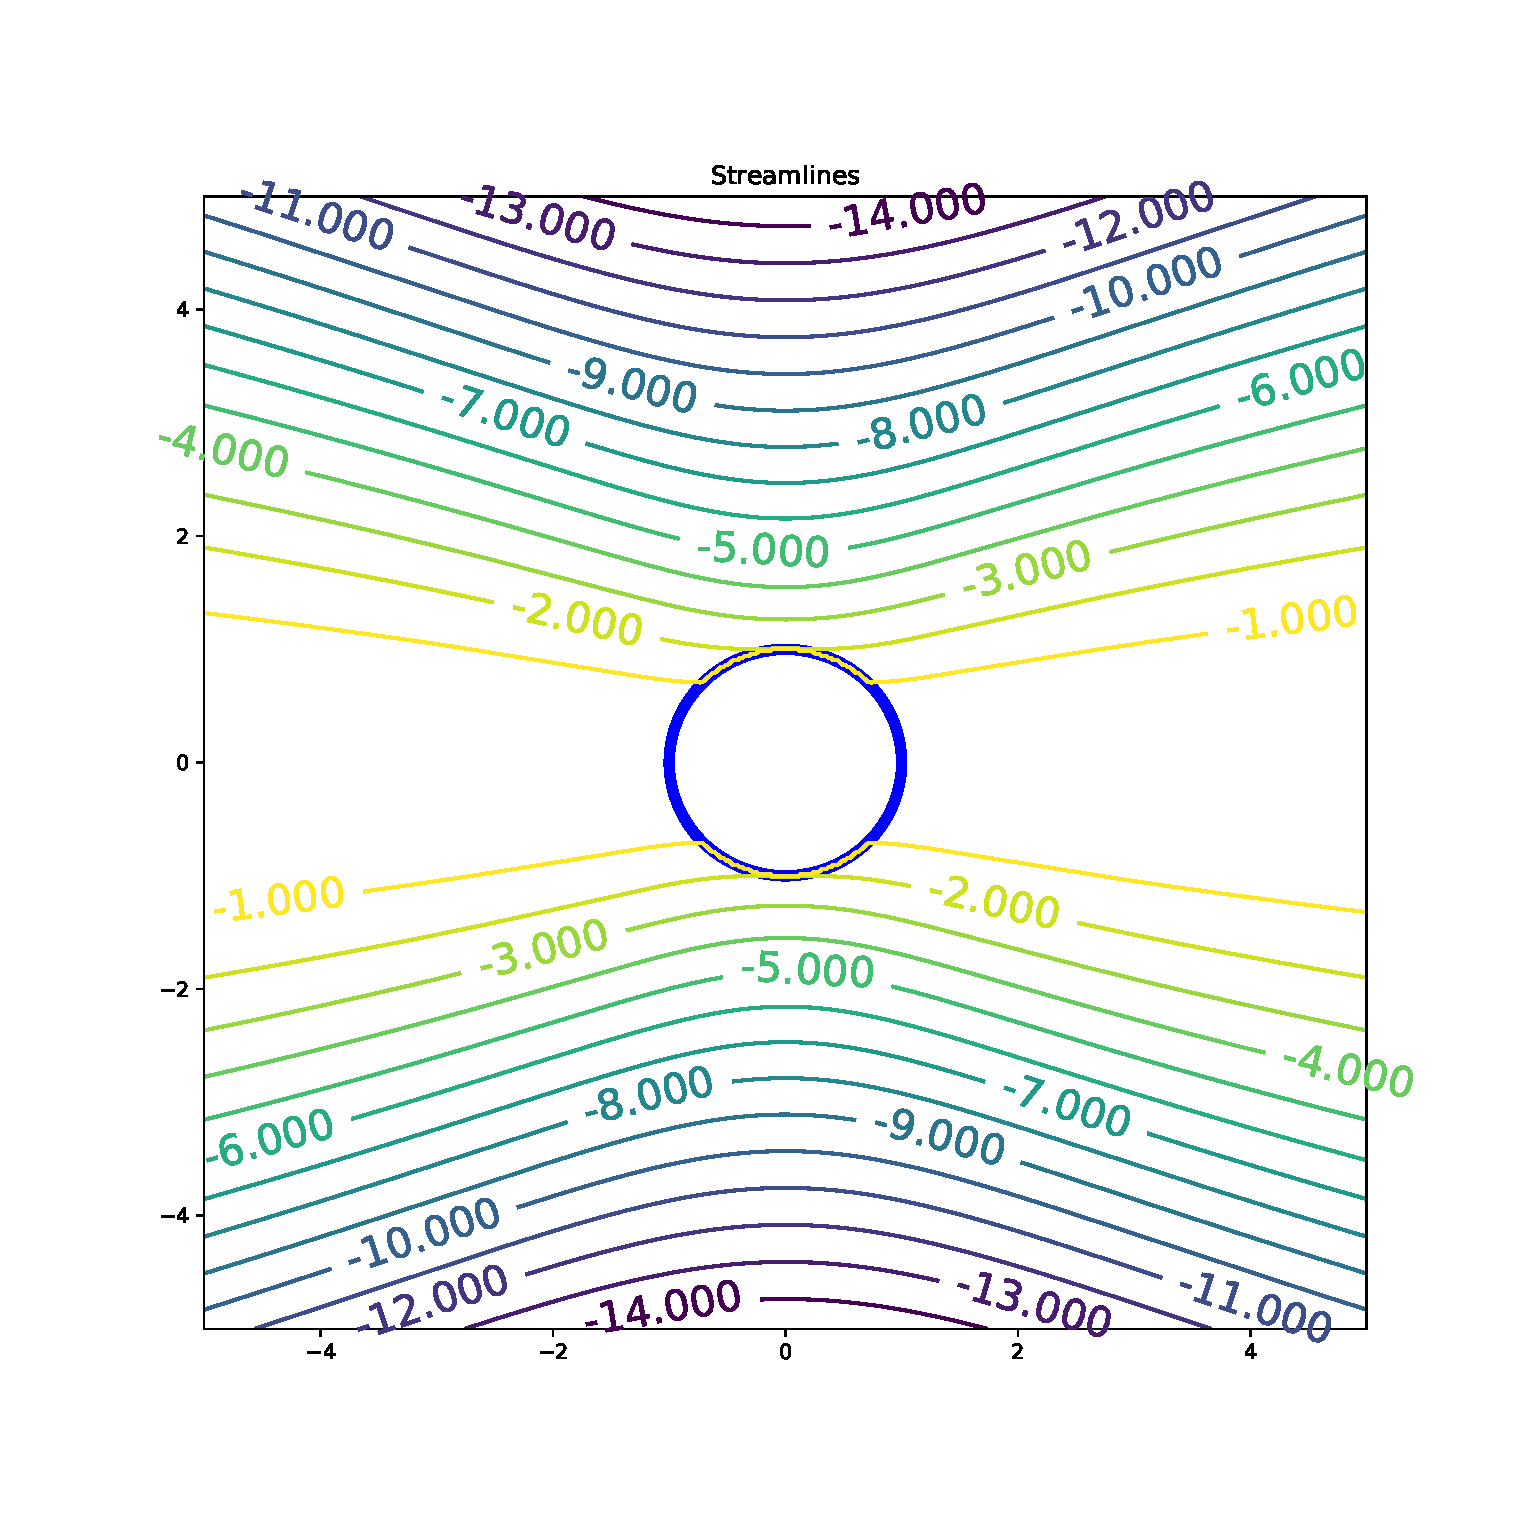
\includegraphics[width=0.8\linewidth]{figures/creeping_flow_past_sphere_moving}
